% !TEX TS-program = xelatex

\documentclass{article}
%\documentclass[landscape]{article}
\def\image{../../../../../Preamble/hselogo.png}

\input{../../../../../Preamble/lepreamble.tex}
\usetikzlibrary{patterns}
\renewcommand{\arraystretch}{1.185}

\pagestyle{fancy} 
\fancyhead{} 
\fancyhead[C]{\large }
\fancyhead[L]{\large \today} 
\fancyhead[R]{\large Плотность и дифференциалы}
\fancyfoot{} 
\fancyfoot[C]{\large \thepage}

\begin{document}
\large
\begin{btitleframe}{\Large Плотность и дифференциалы}
\flushleft{\textbf{Составители:} Александр Югай, Егор Фадеев, Анна Казачкова, Александр Ганибаев} \vspace{-0.6em}
\flushleft{\textbf{Группа:} БЭК181} \vspace{-0.6em}
\flushleft{\textit {\today}}
\vspace{1em}
\end{btitleframe}

\problem{
Точки равномерно распределены на множестве:

\[D=\{(x,\ y):\ x^2+y^2\le R^2\}\]

Найти функции плотности для абсциссы $f_X(x)$ и ординаты $f_{Y}(y)$ точки.
}

\solution{
 Аппроксимируем вероятность попадания $X$ в  интервал $[x, x+dx]$  отношением площади прямоугольника со сторонами $2y$ и $dx$ и площади всего круга $S$.

\begin{center}
    \tikzset{every picture/.style={line width=0.75pt}} %set default line width to 0.75pt        

    \begin{tikzpicture}[x=0.75pt,y=0.75pt,yscale=-1,xscale=1]
    %uncomment if require: \path (0,300); %set diagram left start at 0, and has height of 300

    %Shape: Axis 2D [id:dp9088274993455128] 
    \draw  (356,161.29) -- (632.5,161.29)(495.33,22.5) -- (495.33,299) (625.5,156.29) -- (632.5,161.29) -- (625.5,166.29) (490.33,29.5) -- (495.33,22.5) -- (500.33,29.5)  ;
    %Shape: Circle [id:dp5967966055466523] 
    \draw   (406.46,161.29) .. controls (406.46,112.21) and (446.25,72.42) .. (495.33,72.42) .. controls (544.42,72.42) and (584.21,112.21) .. (584.21,161.29) .. controls (584.21,210.38) and (544.42,250.17) .. (495.33,250.17) .. controls (446.25,250.17) and (406.46,210.38) .. (406.46,161.29) -- cycle ;
    %Shape: Axis 2D [id:dp30032439372877406] 
    \draw  (31,161.29) -- (307.5,161.29)(170.33,22.5) -- (170.33,299) (300.5,156.29) -- (307.5,161.29) -- (300.5,166.29) (165.33,29.5) -- (170.33,22.5) -- (175.33,29.5)  ;
    %Shape: Circle [id:dp7888466377067511] 
    \draw   (81.46,161.29) .. controls (81.46,112.21) and (121.25,72.42) .. (170.33,72.42) .. controls (219.42,72.42) and (259.21,112.21) .. (259.21,161.29) .. controls (259.21,210.38) and (219.42,250.17) .. (170.33,250.17) .. controls (121.25,250.17) and (81.46,210.38) .. (81.46,161.29) -- cycle ;
    %Shape: Rectangle [id:dp6558701777355453] 
    \draw  [dash pattern={on 4.5pt off 4.5pt}] (196.54,76.75) -- (212,76.75) -- (212,245.75) -- (196.54,245.75) -- cycle ;
    %Shape: Brace [id:dp2592467848204758] 
    \draw   (197,77.5) .. controls (192.33,77.5) and (190,79.83) .. (190,84.5) -- (190,109.38) .. controls (190,116.05) and (187.67,119.38) .. (183,119.38) .. controls (187.67,119.38) and (190,122.71) .. (190,129.38)(190,126.38) -- (190,154.25) .. controls (190,158.92) and (192.33,161.25) .. (197,161.25) ;
    %Shape: Rectangle [id:dp47887906958575654] 
    \draw  [dash pattern={on 4.5pt off 4.5pt}] (411.19,130.09) -- (411.14,114.63) -- (580.14,114.07) -- (580.19,129.53) -- cycle ;
    %Shape: Brace [id:dp4633216208147717] 
    \draw   (495.6,130) .. controls (495.6,134.67) and (497.93,137) .. (502.6,137) -- (527.92,137) .. controls (534.59,137) and (537.92,139.33) .. (537.92,144) .. controls (537.92,139.33) and (541.25,137) .. (547.92,137)(544.92,137) -- (573.25,137) .. controls (577.92,137) and (580.25,134.67) .. (580.25,130) ;

    % Text Node
    \draw (636,160.9) node [anchor=north west][inner sep=0.75pt]    {$x$};
    % Text Node
    \draw (477,13.9) node [anchor=north west][inner sep=0.75pt]    {$y$};
    % Text Node
    \draw (311,160.9) node [anchor=north west][inner sep=0.75pt]    {$x$};
    % Text Node
    \draw (152,13.9) node [anchor=north west][inner sep=0.75pt]    {$y$};
    % Text Node
    \draw (201,58.4) node [anchor=north west][inner sep=0.75pt]  [font=\small]  {$dx$};
    % Text Node
    \draw (171,106.9) node [anchor=north west][inner sep=0.75pt]  [font=\small]  {$y$};
    % Text Node
    \draw (182,160.9) node [anchor=north west][inner sep=0.75pt]  [font=\small]  {$x$};
    % Text Node
    \draw (213,160.9) node [anchor=north west][inner sep=0.75pt]  [font=\small]  {$x+dx$};
    % Text Node
    \draw (480.8,132.8) node [anchor=north west][inner sep=0.75pt]  [font=\small]  {$y$};
    % Text Node
    \draw (454.4,96) node [anchor=north west][inner sep=0.75pt]  [font=\small]  {$y+dy$};
    % Text Node
    \draw (533.55,141.3) node [anchor=north west][inner sep=0.75pt]  [font=\small]  {$x$};

    \draw [fill={rgb, 255:red, 0; green, 0; blue, 0 }  ,fill opacity=1 ]  (212, 161.29) circle [x radius= 2, y radius= 2]   ;
    \draw [fill={rgb, 255:red, 0; green, 0; blue, 0 }  ,fill opacity=1 ]  (196.54, 161.29) circle [x radius= 2, y radius= 2]   ;
    \draw [fill={rgb, 255:red, 0; green, 0; blue, 0 }  ,fill opacity=1 ]  (495.33, 114.35) circle [x radius= 2, y radius= 2]   ;
    \draw [fill={rgb, 255:red, 0; green, 0; blue, 0 }  ,fill opacity=1 ]  (495.33, 129.81) circle [x radius= 2, y radius= 2]   ;
    \end{tikzpicture}
\end{center}

\begin{align}
    &x^2+y^2=R^2 & S=\pi R^2\\
    &y=\sqrt{R^2-x^2} &
\end{align}

\begin{align}
    P(X\in [x, x+dx]) &= \frac{2\sqrt{R^2-x^2}}{\pi R^2}dx + o(dx)
\end{align}

\[
        f_X(x) = \begin{cases}
        \dfrac{2\sqrt{R^2-x^2}}{\pi R^2},\ &x \in [-R, R]\\
        0,\ &x \notin [-R, R]
    \end{cases}
\]

Для ординаты функция плотности находится аналогично.

\[
        f_Y(y) = \begin{cases}
        \dfrac{2\sqrt{R^2-y^2}}{\pi R^2}\, & y \in [-R, R]\\
        0\, & y \notin [-R, R]
    \end{cases}
\]
}

\problem{
Точки равномерно распределены на области, ограниченной прямыми $y=1-x,\ x=0,\ y=0$. Найти функции плотности для абсциссы $f_X(x)$ и ординаты $f_{Y}(y)$ точки.
}

\solution{
 Аппроксимируем вероятность попадания $X$ в интервал $[x, x+dx]$ отношением площади прямоугольника со сторонами $y$ и $dx$ и площади всего треугольника $S$.
 
\begin{center}
    \begin{tikzpicture}[x=0.75pt,y=0.75pt,yscale=-1,xscale=1]
    %uncomment if require: \path (0,300); %set diagram left start at 0, and has height of 300

    %Shape: Axis 2D [id:dp30032439372877406] 
    \draw  (191,259.2) -- (467.5,259.2)(233.4,14.5) -- (233.4,291) (460.5,254.2) -- (467.5,259.2) -- (460.5,264.2) (228.4,21.5) -- (233.4,14.5) -- (238.4,21.5)  ;
    %Shape: Rectangle [id:dp6558701777355453] 
    \draw  [dash pattern={on 4.5pt off 4.5pt}] (280.94,158) -- (296.4,158) -- (296.4,258.95) -- (280.94,258.95) -- cycle ;
    %Straight Lines [id:da9117461569714944] 
    \draw    (226.2,102.8) -- (389.4,266) ;
    %Shape: Rectangle [id:dp17972359402967553] 
    \draw  [dash pattern={on 4.5pt off 4.5pt}] (339.08,200.33) -- (339.21,215.79) -- (233.86,216.65) -- (233.73,201.2) -- cycle ;

    % Text Node
    \draw (471,262.35) node [anchor=north west][inner sep=0.75pt]    {$x$};
    % Text Node
    \draw (215.6,-2.5) node [anchor=north west][inner sep=0.75pt]    {$y$};
    % Text Node
    \draw (268.4,263.15) node [anchor=north west][inner sep=0.75pt]  {$x$};
    % Text Node
    \draw (298.4,262.35) node [anchor=north west][inner sep=0.75pt]  {$x+dx$};
    % Text Node
    \draw (239.2,93) node [anchor=north west][inner sep=0.75pt]  {$1$};
    % Text Node
    \draw (386,240.6) node [anchor=north west][inner sep=0.75pt]  {$1$};
    % Text Node
    \draw (190.4,184.6) node [anchor=north west][inner sep=0.75pt]  {$y+dy$};
    % Text Node
    \draw (218.8,215) node [anchor=north west][inner sep=0.75pt]  {$y$};

    \draw [fill={rgb, 255:red, 0; green, 0; blue, 0 }  ,fill opacity=1 ]  (382.6, 259.2) circle [x radius= 2, y radius= 2]   ;
    \draw [fill={rgb, 255:red, 0; green, 0; blue, 0 }  ,fill opacity=1 ]  (233.4, 110) circle [x radius= 2, y radius= 2]   ;
    \end{tikzpicture}
\end{center}
 
\begin{align}
    y &= 1-x\\
    S &= \frac{1}{2}\cdot 1 \cdot 1 =\frac{1}{2}
\end{align}

\[
    P(X\in [x, x+dx]) = \frac{1-x}{1/2}dx + o(dx)= 2(1-x)dx + o(dx)
\]

\[
        f_X(x) = \begin{cases}
        2(1-x),\ &x \in [0, 1]\\
        0,\ &x \notin [0, 1]
    \end{cases}
\]

Для ординаты функция плотности находится аналогично.

\[
        f_Y(y) = \begin{cases}
        2(1-y),\ &y \in [0, 1]\\
        0,\ &y \notin [0, 1]
    \end{cases}
\]
}

\problem{
Точки равномерно распределены на области, ограниченной кривыми $\ln{x+1}, x=1, y=0$. Найти функции плотности для абсциссы $f_X(x)$ и ординаты $f_{Y}(y)$ точки.
}

\solution{
    Аппроксимируем вероятность попадания $X$ в интервал $[x, x+dx]$ отношением площади прямоугольника со сторонами $y$ и $dx$ и площади всей фигуры $S$.
    
    \begin{center}
        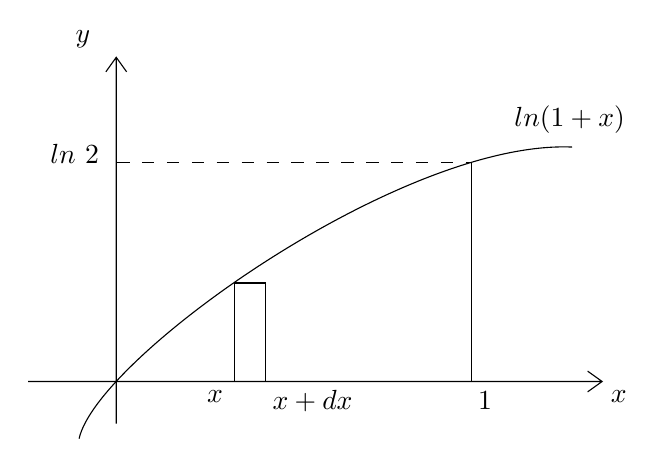
\begin{tikzpicture}[x=0.75pt,y=0.75pt,yscale=-1,xscale=1]
        %uncomment if require: \path (0,300); %set diagram left start at 0, and has height of 300

        %Shape: Axis 2D [id:dp30032439372877406] 
        \draw  (191,270.7) -- (467.5,270.7)(233.4,114.5) -- (233.4,291) (460.5,265.7) -- (467.5,270.7) -- (460.5,275.7) (228.4,121.5) -- (233.4,114.5) -- (238.4,121.5)  ;
        %Curve Lines [id:da07393987701751148] 
        \draw    (215.5,298.25) .. controls (224,259.25) and (371,154.25) .. (453,157.75) ;
        %Shape: Rectangle [id:dp9272591150725811] 
        \draw   (290.5,223.25) -- (305.5,223.25) -- (305.5,270.5) -- (290.5,270.5) -- cycle ;
        %Straight Lines [id:da6532183868024182] 
        \draw    (404.5,165) -- (404.5,270.75) ;
        %Straight Lines [id:da1919337674414925] 
        \draw  [dash pattern={on 4.5pt off 4.5pt}]  (233.8,165) -- (404.5,165) ;

        % Text Node
        \draw (470.5,273.6) node [anchor=north west][inner sep=0.75pt]    {$x$};
        % Text Node
        \draw (212.6,100.5) node [anchor=north west][inner sep=0.75pt]    {$y$};
        % Text Node
        \draw (275.9,273.6) node [anchor=north west][inner sep=0.75pt]  [font=\normalsize]  {$x$};
        % Text Node
        \draw (307.5,273.9) node [anchor=north west][inner sep=0.75pt]  [font=\normalsize]  {$x+dx$};
        % Text Node
        \draw (406.5,274.15) node [anchor=north west][inner sep=0.75pt]    {$1$};
        % Text Node
        \draw (200.4,155.1) node [anchor=north west][inner sep=0.75pt]    {$ln\ 2$};
        % Text Node
        \draw (424,136.7) node [anchor=north west][inner sep=0.75pt]    {$ln( 1+x)$};


        \end{tikzpicture}
    \end{center}

    \[
        S = \int\limits_{0}^1 \ln{1+x}dx 
    \]
    
    \begin{multline}
        \int \ln{1+x}dx=x\ln{1+x}-\int\frac{x}{x+1}dx=\\
        =x\ln{1+x}-\int\frac{x+1}{x+1}dx+\int\frac{1}{x+1}dx=\\
        =x\ln{1+x}-x+\ln{1+x}=(1+x)\ln{1+x}-x
    \end{multline}
    \begin{align}
        S&=\left.(1+x)\ln{1+x}-x\right|_{0}^1=2\ln2-1\\
        y&=\ln{1+x}
    \end{align}
    
    \[
        P(X\in [x, x+dx]) = \frac{\ln{1+x}}{2\ln2-1}dx+o(dx)
    \]
    
    \[
        f_X(x) = \begin{cases}
        \dfrac{\ln{1+x}}{2\ln2-1},\ &x \in [0, 1]\\
        0,\ &x \notin [0, 1]
    \end{cases}
    \]

    \begin{center}
        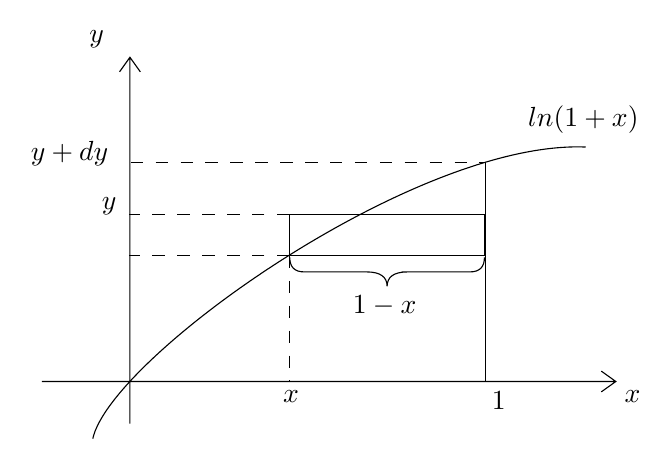
\begin{tikzpicture}[x=0.75pt,y=0.75pt,yscale=-1,xscale=1]
        %uncomment if require: \path (0,300); %set diagram left start at 0, and has height of 300
        
        %Shape: Axis 2D [id:dp30032439372877406] 
        \draw  (191,270.7) -- (467.5,270.7)(233.4,114.5) -- (233.4,291) (460.5,265.7) -- (467.5,270.7) -- (460.5,275.7) (228.4,121.5) -- (233.4,114.5) -- (238.4,121.5)  ;
        %Curve Lines [id:da07393987701751148] 
        \draw    (215.5,298.25) .. controls (224,259.25) and (371,154.25) .. (453,157.75) ;
        %Shape: Rectangle [id:dp9272591150725811] 
        \draw   (310.2,190.2) -- (404.2,190.2) -- (404.2,210.2) -- (310.2,210.2) -- cycle ;
        %Straight Lines [id:da6532183868024182] 
        \draw    (404.5,165) -- (404.5,270.75) ;
        %Straight Lines [id:da1919337674414925] 
        \draw  [dash pattern={on 4.5pt off 4.5pt}]  (233.8,165) -- (404.5,165) ;
        %Shape: Brace [id:dp7565439725942462] 
        \draw   (310.4,210.9) .. controls (310.4,215.57) and (312.73,217.9) .. (317.4,217.9) -- (347.3,217.9) .. controls (353.97,217.9) and (357.3,220.23) .. (357.3,224.9) .. controls (357.3,220.23) and (360.63,217.9) .. (367.3,217.9)(364.3,217.9) -- (397.2,217.9) .. controls (401.87,217.9) and (404.2,215.57) .. (404.2,210.9) ;
        %Straight Lines [id:da15576293614395076] 
        \draw  [dash pattern={on 4.5pt off 4.5pt}]  (310.2,210.2) -- (310.2,270.8) ;
        %Straight Lines [id:da4419318213939003] 
        \draw  [dash pattern={on 4.5pt off 4.5pt}]  (310.2,190.2) -- (233,190.2) ;
        %Straight Lines [id:da06118190882704111] 
        \draw  [dash pattern={on 4.5pt off 4.5pt}]  (310.2,210.2) -- (233,210.2) ;
        
        % Text Node
        \draw (470.5,273.6) node [anchor=north west][inner sep=0.75pt]    {$x$};
        % Text Node
        \draw (212.6,100.5) node [anchor=north west][inner sep=0.75pt]    {$y$};
        % Text Node
        \draw (305.9,273.6) node [anchor=north west][inner sep=0.75pt]  [font=\normalsize]  {$x$};
        % Text Node
        \draw (406.5,274.15) node [anchor=north west][inner sep=0.75pt]    {$1$};
        % Text Node
        \draw (424,136.7) node [anchor=north west][inner sep=0.75pt]    {$ln( 1+x)$};
        % Text Node
        \draw (339.6,227.9) node [anchor=north west][inner sep=0.75pt]    {$1-x$};
        % Text Node
        \draw (184.4,153.9) node [anchor=north west][inner sep=0.75pt]    {$y+dy$};
        % Text Node
        \draw (218.6,180.9) node [anchor=north west][inner sep=0.75pt]    {$y$};
        
        
        \end{tikzpicture}
    \end{center}
        
Аппроксимируем вероятность попадания $Y$ в интервал $[y\cm y+dy]$ отношением площади прямоугольника со сторонами $(1-x)$ и $dy$ и площади всей фигуры $S$.

    
    
    \begin{align}
        y = \ln{1+x}\\
        e^y = 1+x\\
        1-x = 2-e^y
    \end{align}
    
    \[
        P(Y\in [y, y+dy]) = \frac{2-e^y}{2\ln2-1}dy+o(dy)
    \]
    
    \[
        f_Y(y) = \begin{cases}
        \dfrac{2-e^y}{2\ln2-1},\ &y \in [0, \ln2]\\
        0,\ &y \notin [0, \ln2]
    \end{cases}
    \]
}

\problem{
Заданы множества:

\begin{align}
    D_1 = \{(x,y): x^2+y^2 \le 4\} && D_2 = \{(x,y): (x-1)^2+y^2 \le 3\}
\end{align}

Точки равномерно распределены в множестве $A = D_1 \setminus D_2$. Найти функции плотности для абсциссы $f_X(x)$ и ординаты $f_{Y}(y)$ точки.
}

\problem{
Найти функции плотности $x$ и $y$ на фигуре, ограниченной кривыми $x = 0$, $y = e^x$ и $y = x^2$.
}

\solution{
Для начала можно разбить фигуру на две части. Для этого найдем точку пересечения кривых $e^x$ и $x^2$. Приравняв их, получаем некоторый $x = a = const$. В зависимости от того, чем уравен x относительно a, будут меняться функции плотности для обеих величин.

Пусть площадь фигуры равна S. Чтобы найти функции плотности через о-малое, будем находить отношение площади прямоугольника с парметрами dx и y к площади всей фигуры, для y аналогичным способом.

\begin{align*}
f_X(x) =
\begin{cases}
\frac{e^x}{S}; & x \textless a\\
\frac{x^2}{S}; & x\geqslant a\\
\end{cases}
\end{align*}

\begin{align*}
f_Y(x, y) =
\begin{cases}
\frac{\sqrt{y}}{S}; & x \textless a\\
\frac{lny}{S}; & x\geqslant a\\
\end{cases}
\end{align*}
\begin{center}
    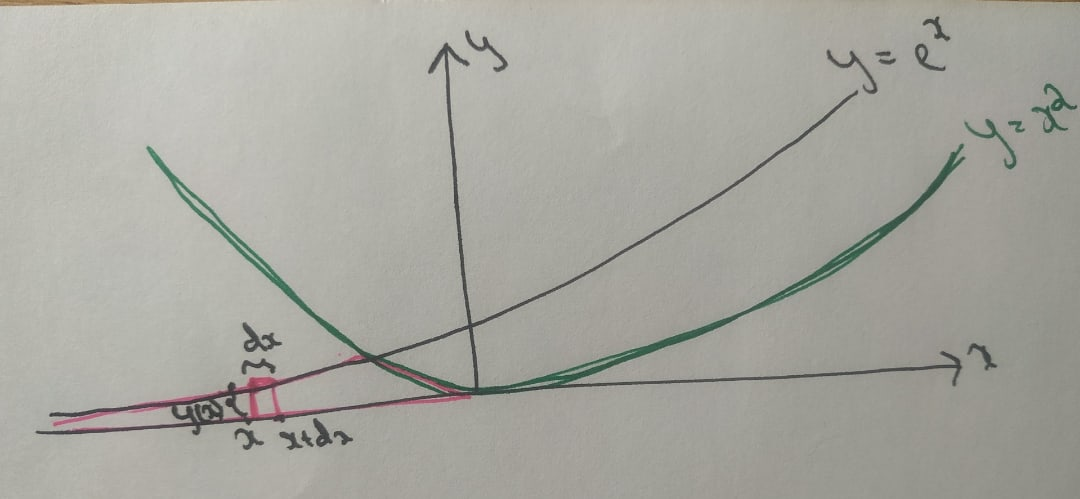
\includegraphics[width=0.8\textwidth]{6}
\end{center}
}

\problem{
Найти функцию плотности $x$ на фигуре, ограниченной кривыми $y=x^5$, $y=0$, $x=2$.
}

\solution{
Площадь фигуры можно найти через интеграл, она получается равной $\frac{32}{3}$.

Функция плотности находится как отношение аппроксимированной вероятности попадания на определенную координату x ко всей площади фигуры. Получается:
\begin{align*}
f_X(x) =
\begin{cases}
\frac{x^5}{\frac{32}{3}}; & x \in [0; 2]\\
0; & else\\
\end{cases}
\end{align*}
\begin{center}
    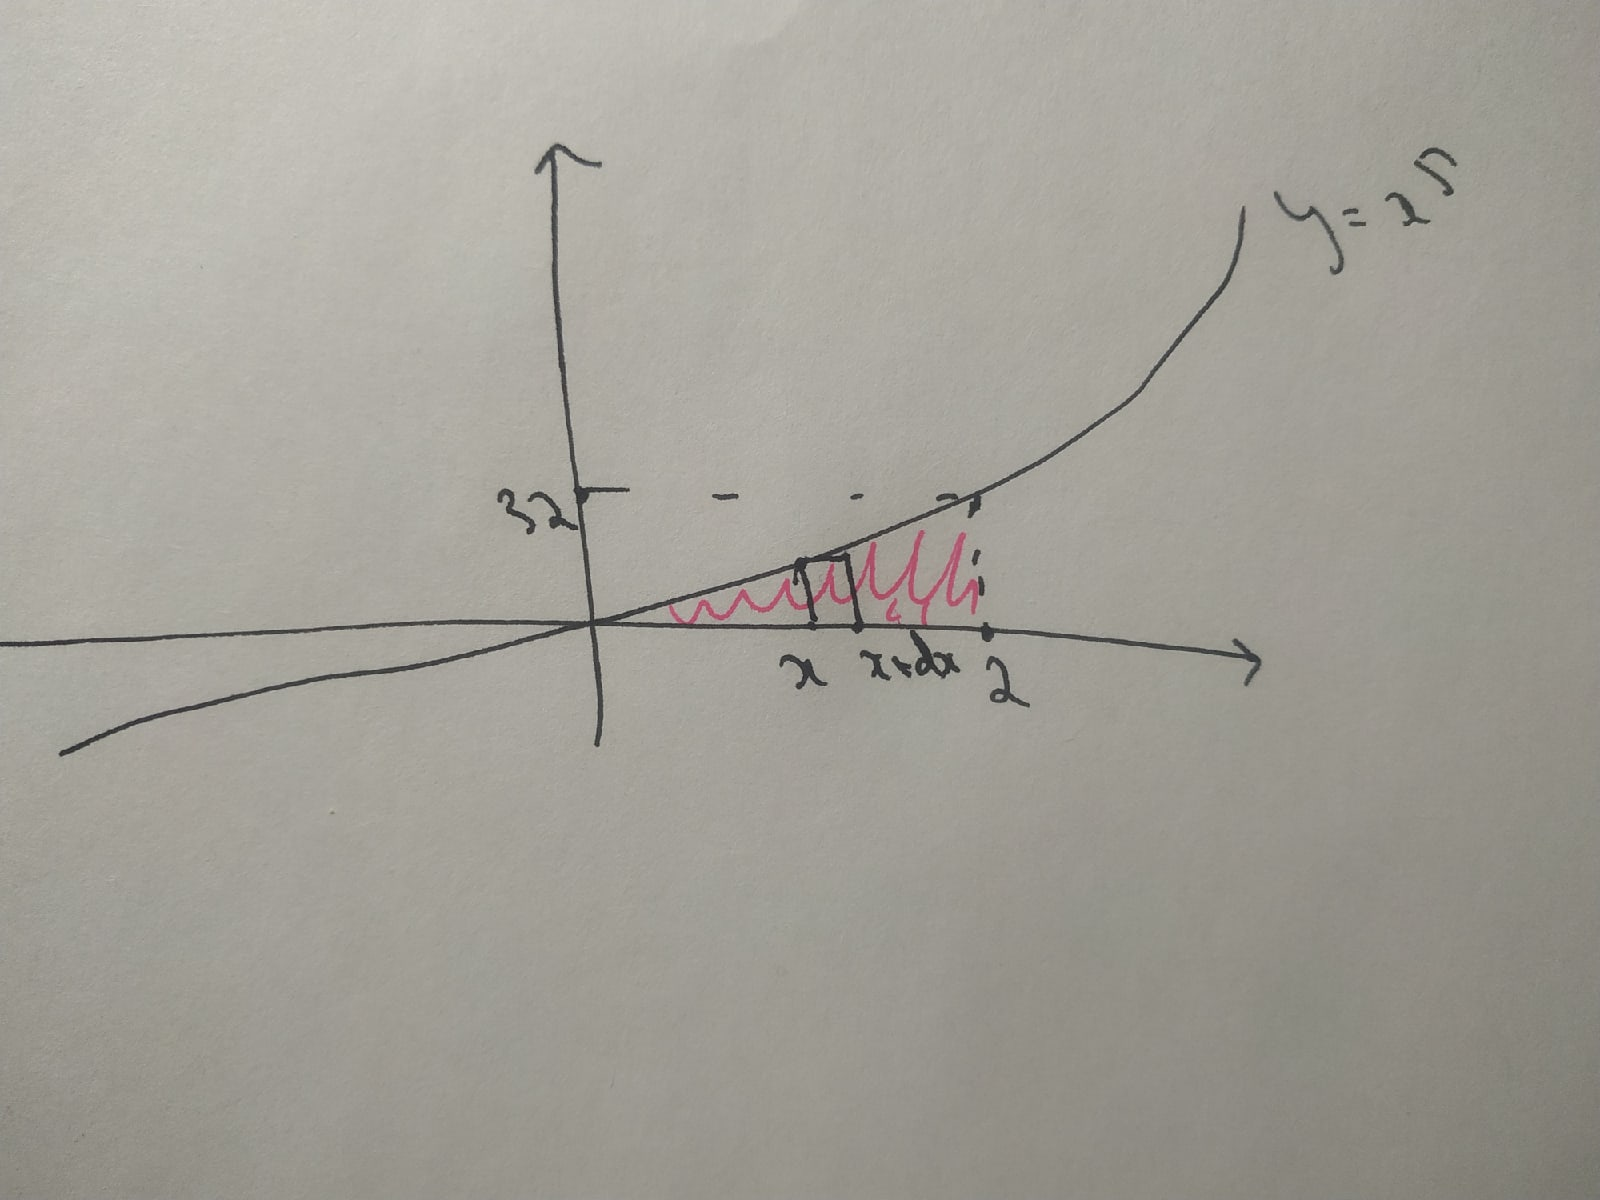
\includegraphics[width=0.8\textwidth]{7}
\end{center}
}

\problem{
Найти функцию плотности $x$ на фигуре, ограниченной прямыми $y = 0$, $y=x$ и $y =-x+2$.
}

\solution{
Площадь фигуры получается равной 1. Функция плотности находится путем аналогичной аппроксимации вероятности попадения в определенную точку. Получается:
\begin{align*}
f_X(x) =
\begin{cases}
x; & x \in [0;1]\\
-x +2; & else\\
\end{cases}
\end{align*}
\begin{center}
    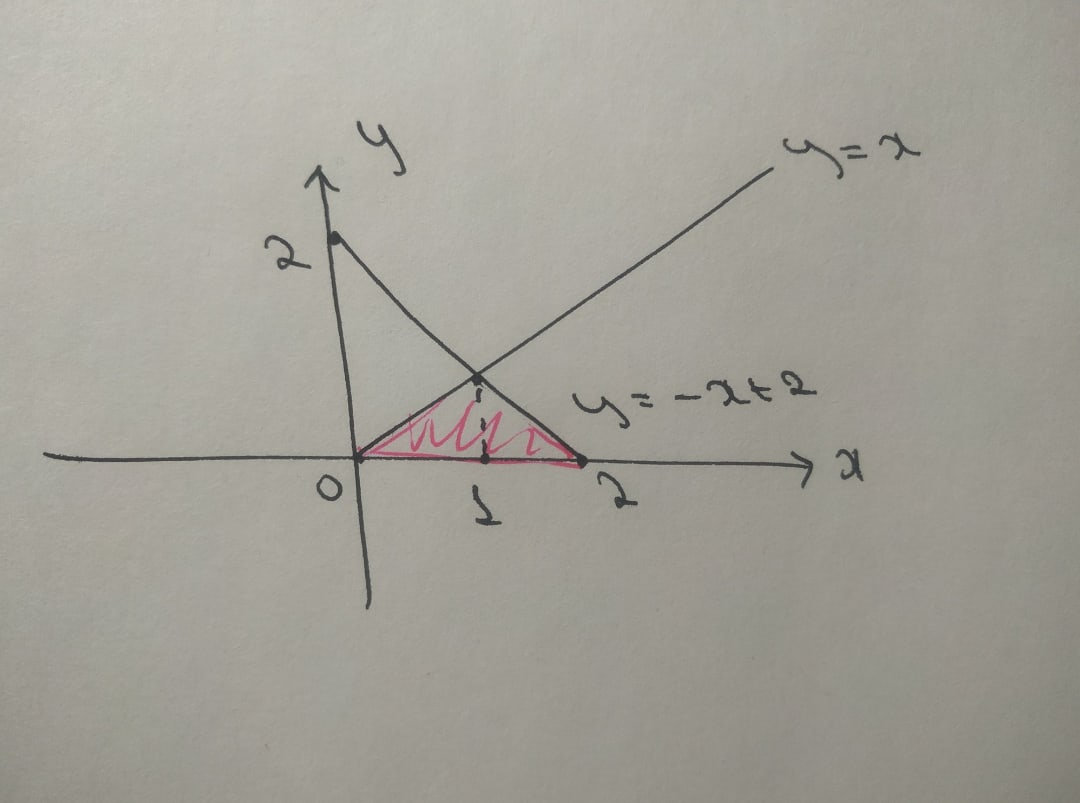
\includegraphics[width=0.8\textwidth]{8}
\end{center}
}

%%%%%%%%%%%%%

\problem{
    Точки равномерно распределены на области, ограниченной кривыми $y=-(x-1)^2+1,\ y=0$. Найти функции плотности для абсциссы $f_X(x)$ и ординаты $f_{Y}(y)$ точки.
}

\solution{
    Аппроксимируем вероятность попадания $X$ в интервал $[x, x+dx]$ отношением площади прямоугольника со сторонами $y$ и $dx$ и площади всей фигуры $S$.
    \begin{center}
        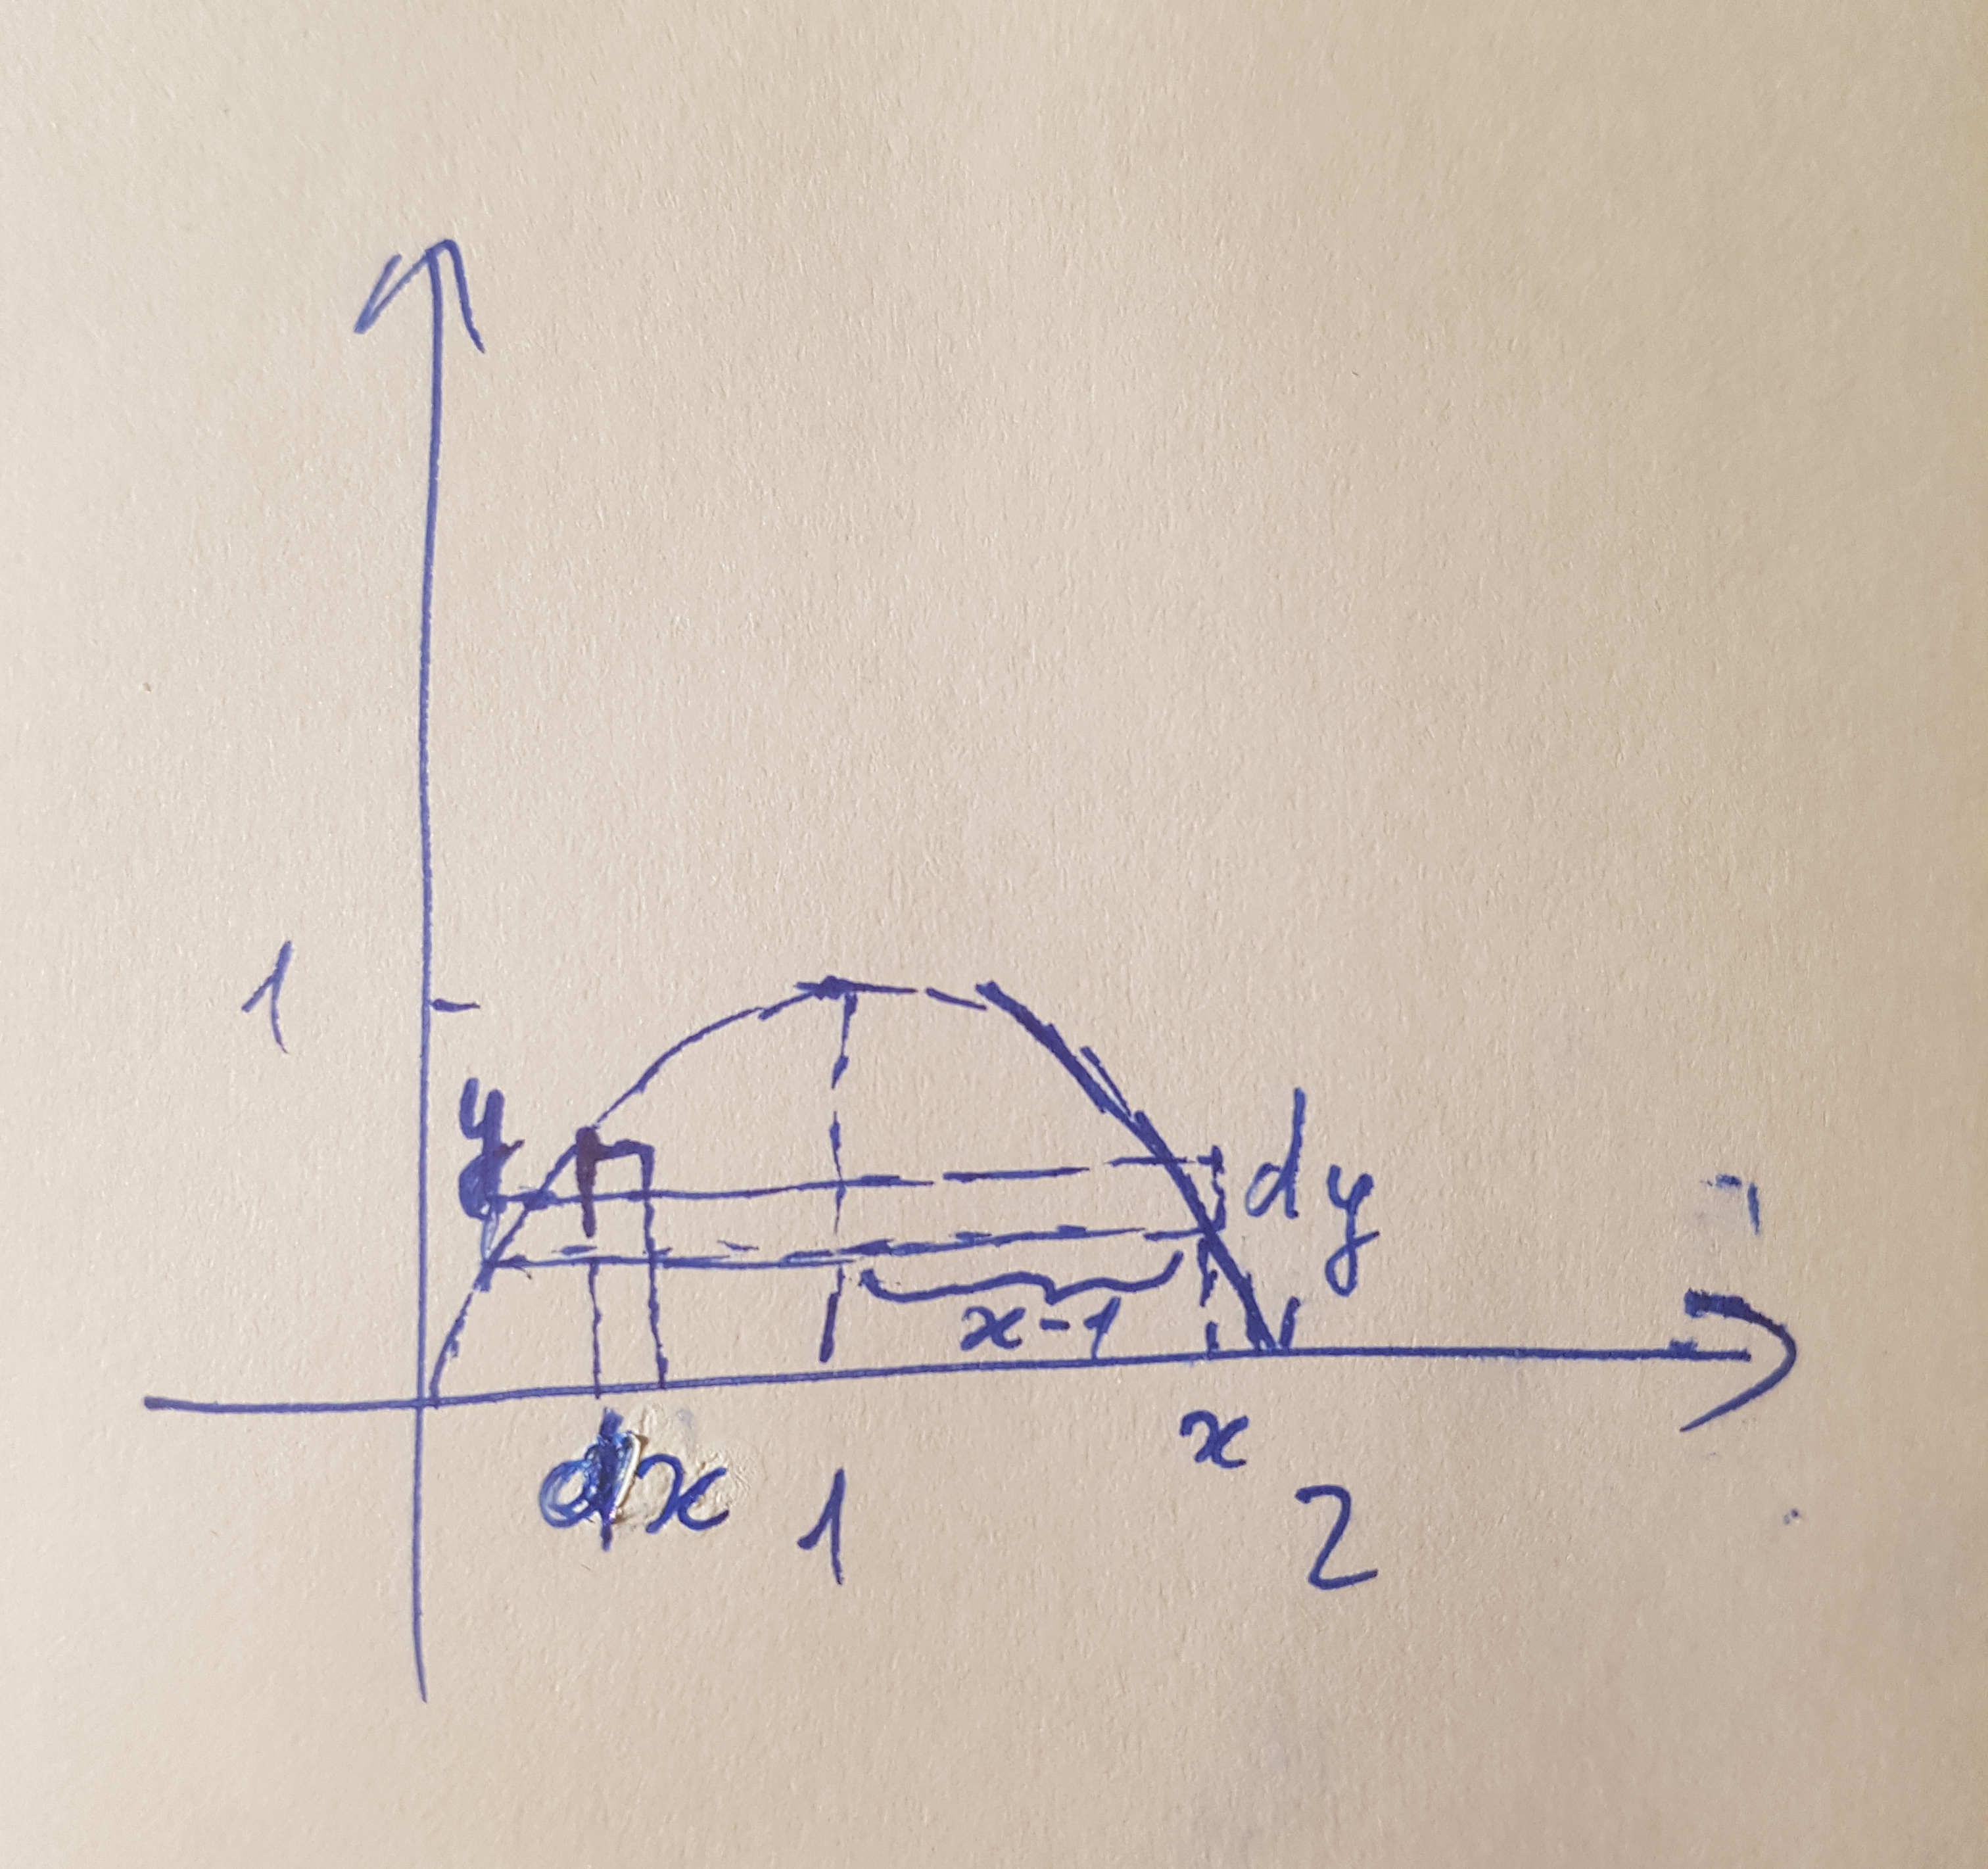
\includegraphics[width=0.8\textwidth]{5.jpg}
    \end{center}
    
    \begin{multline}
        S = \int\limits_{0}^2 (-(x-1)^2+1)dx = \\
        =\int\limits_{0}^2 (-(x-1)^2+1)d(x-1)=\\
        =\left.\frac{-(x-1)^3}{3}+x-1\right|_{0}^2 = -\frac{1}{3}+2-1-\frac{1}{3}+1= \frac{4}{3}
    \end{multline}
    \[
        P(X\in [x, x+dx]) = \frac{(1-(x-1)^2)}{4/3}dx+o(dx)
    \]
    
    \begin{equation}
        f_X(x) = \begin{cases}
        \dfrac{3(1-(x-1)^2)}{4},\ &x \in [0, 2]\\
        0,\ &x \notin [0, 2]
    \end{cases}
    \end{equation}
    Аппроксимируем вероятность попадания $Y$ в интервал $[y, y+dy]$ отношением площади прямоугольника со сторонами $2(x-1)$ и $dy$ и площади всей фигуры $S$.
    
    \begin{align}
        y=1-(x-1)^2\\
        x-1 = \sqrt{1-y} 
    \end{align}
    \[
        P(Y\in [y, y+dy]) = \frac{2\sqrt{1-y}}{4/3}dy+o(dy)
    \]
    
    \begin{equation}
        f_Y(y) = \begin{cases}
        \dfrac{3\sqrt{1-y}}{2}, &y \in [0, 1]\\
        0, &y \notin [0, 1]
    \end{cases}
    \end{equation}
}

\problem{
    Две точки равномерно распределены на окружности с центром в начале координат и радиусом $R$. Найти плотность распределения расстояния между двумя точками.
}

\solution{
    Немного переформулируем условие. Пусть координаты первой точки всегда $(-1, 0)$, а вторая точка равномерно распределена на окружности. Тогда $\alpha$ - наименьший угол между радиусами, проведенных к точкам, причем:
    
    \[
        \alp \sim U[0, \pi]
    \]
    
    Тогда расстояние $D$ между точками выразить через $\alp$ и $R$, используя теорему косинусов:
    \[
        D^2 = R^2+R^2-2R^2\cos{\alp}        
    \] 
}

\end{document}
